\section{Introduction}
\label{sec:introduction}

The rapid progress in the field of generative AI and the now widespread access to advanced AI tools like ChatGPT
 have unleashed a new wave of speculations on how industries are going to evolve over the next few years, see,
 e.g., \cite{chuiHowGenerativeAI2022,chuiWhatEveryCEO2023}. Many companies are reconsidering how 
AI in general and generative AI in particular will affect their industries and ecosystems. One such industry is
career counseling, which is also known as career guidance. Career counseling is the discipline and set of services
related to designing career paths and consulting individuals regarding their career opportunities.
In this paper we explore a new innovative business model in career counseling based on co-creation that we term
\textit{Career-Counseling-as-a-Service} (CCaaS). We envisage CCaaS as a set of next-generation, AI-powered career
counseling services that are offered as an API-based solution. This new business model is embedded in a social and
digital ecosystem of career counseling by leveraging the vast amount of data of the most powerful company in terms
of professionals' career data, i.e., LinkedIn\footnote[1]{\url{https://www.linkedin.com}} and will enable new types
of value co-creation by different actors in the ecosystem.

Digital ecosystems can be described as a complex, self-organizing, and adaptive system of actors (including current and
potential competitors) and other stakeholders that are connected through digital platforms in order to create and exchange
value. More specifically, \cite{adnerEcosystemStructureActionable2017} defines an ecosystem as follows: an \textit{``[...]
ecosystem is defined by the alignment structure of the multilateral set of partners that need to interact in order for a
focal value proposition to materialize.''} By alignment structure, Adner refers to the mutual understanding and agreement
of the position of different actors in the ecosystem, i.e., the roles they play and the relationships they have with each other
\citep[p. 42]{adnerEcosystemStructureActionable2017}. While by ``multilateral'' and ``set of partners'' Adner refers to
the fact that the ecosystems are composed of a multitude of actors, but also that these actors are members of the ecosystem
and share the same goal of a joint value creation \citep[p. 42-43]{adnerEcosystemStructureActionable2017}. Digital ecosystems
have gained tremendous importance over the last few years and translate into business growth and accrued financial success
for companies \citep{weillThrivingIncreasinglyDigital2015}.

The remainder of the paper is built as follows. We will first introduce the customer perspective on career counseling
before developing the value proposition using the Value Proposition Canvas \citep{osterwalderValuePropositionDesign2014}.
In particular, in Section \ref{sec:customer_perspective} we will look at the customer perspective in terms of possible
customer segments and their respective needs and drivers. Needs to encompass \textit{gains} and \textit{pains} of the
customer segments, while drivers encompass societal, technological and environmental trends and developments that make
this business model possible. Further, we will describe the enablers of this new business model. Enablers encompass 
the resources available to the innovating company thereby increasing the likelihood of realization and viability of the
new business model, and are described in Section \ref{sec:enablers}. Then, we will describe the business model itself
using the Business Model Canvas \citep{osterwalderBusinessModelGeneration2010} in Section \ref{sec:business_model}.
In particular, we will look at the value proposition, customer segments, channels, customer relationships, key
resources, key activities, key partnerships, revenue streams, and cost structure of this business model.
Further, we will detail the specific contribution of (strategic) innovation in this business model in Section
\ref{sec:contribution}. We will then evaluate the business model in terms of its viability and feasibility in Section
\ref{sec:evaluation}. Finally, we will describe the fit of this business model with the system in which it is embedded
in Section \ref{sec:system_fit}, and conclude with a summary of our findings in Section \ref{sec:conclusion}.

In the remainder of this section, we will give a background on career counseling as well as the strategic
innovation potential that stems from the latest generation of AI technologies applied to this industry. This 
background information is based on the previous results of a literature review conducted as part of the course
``Strategic Business Innovation'' at the University of Applied Sciences and Arts Northwestern Switzerland (FHNW)
\citep{kaserAIpoweredCareerCounseling2023}.

\subsection{Career Counseling}

Career counseling entails the discipline and set of services related to designing career paths and consulting
clients regarding their career opportunities. It is provided by career counselors, which are professionals that
are typically trained in psychology, counseling, and career development. A career counselor's job is to assess 
a client's individual preferences, intelligence, skill sets, work values, and experience in order to help them
find a suitable career path under consideration of the current educational, work, and community contexts
\citep{americanpsychologicalassociationCareerCounseling}. Career counseling services are typically demanded by
three groups: (1) individuals that are in the process of choosing a career, i.e., students that are about to enter
the job market; (2) individuals that are in the process of optimizing or entirely changing their career, i.e.,
by changing into a different role or different industry; and (3) unemployed individuals that are in the process
of reintegrating the job market. Further, in this paper will argue for another customer segment, namely companies
engaged in the ``war for talent'' that are looking for ways to \textit{retain} and further develop talent that
already works for them. Although they are not direct beneficiaries of career counseling services, they are
indirect beneficiaries in the sense that they benefit from the increased productivity and satisfaction of their
employees.

Services in career counseling specifically include services in five areas: (1) career assessment, (2) development
\& training, (3) job search assistance, (4) career transitions, and (5) entrepreuneurship-related services.
\textit{Career assessment} services entail the assessment of the traits of the client, including identifying their
preferences, strengths, skills, and values and matching those with suitable career paths. \textit{Development
\& training} services entail the development of the client's skills and competencies in order to prepare them
for a specific career path or fill skill gaps. \textit{Job search assistance} services entail assisting clients
in finding a job, including identifying suitable job opportunities, preparing for job interviews, and writing
job applications. \textit{Career transition} services entail planning and guiding clients through a transition
into a new role and/or career path, including identifying suitable career paths. Finally, with
\textit{entrepreuneurship-related services} counselors support clients in starting a business, including identifying
suitable business opportunities, writing business plans, and assisting with incorporation. Entrepreuneurship-related
services within career counseling are typically offered by career counselors in job centers as one possible way to
reintegrate unemployed individuals.

\subsection{AI in Career Counseling}

The use of technological innovation and AI in career counseling has been researched before. According to
\cite{westmanArtificialIntelligenceCareer2021} and cited in \cite{kaserAIpoweredCareerCounseling2023}, applying
technological innovation in career counseling can lead to the following benefits: \textit{``improved accessibility,
increased access to information, automating assessments and coaching, network effects (e.g., on multisided platforms),
improved cost-effectiveness, and new types of services''}.

Further, \cite{westmanArtificialIntelligenceCareer2021} identified that AI could play a number of roles in career
counseling in the educational setting of schools and universities where students are in the process of choosing a career
path. They identified four roles for AI, including as coach, collaborator, assistant, and tool \citep{westmanArtificialIntelligenceCareer2021}.
By \textit{AI as coach} they refer to the use of AI as a virtual coach to provide career counseling services to clients; by
\textit{AI as collaborator} they refer to the use of AI to support career counselors in their work as a joint team; by
\textit{AI as assistant} they refer to counselors using AI in specific areas and validating the AI results on a case-by-case
basis; finally, by \textit{AI as tool} they refer to the use of AI for single, narrowly defined tasks, such as a job recommendation
engine based on a client's skills profile \citep{westmanArtificialIntelligenceCareer2021}.

\subsection{Digital Ecosystem of Career Counseling}
\label{subsec:ecosystem}

The digital ecosystem of career counseling is composed of a multitude of actors, including career counselors, clients,
and companies. Career counselors are the service providers, whilst clients are the recipients of career counseling services.
Companies can either be beneficiaries of the services that career counselors provide to clients, or they can actively engage
as a member of the digital ecosystem surrounding career counseling. Such members may offer digital platforms and services
that are used by career counselors, clients, or both. The most prominent example of such a platform is LinkedIn, which
is primarily used by clients as a professional social network and to find jobs. Parts of the current ecosystem surrounding
LinkedIn are depicted in Figure \ref{fig:ecosystem}. Other types of platforms include specialized job search engines (such as
Indeed and Glassdoor), career assessment platforms (such as ChoiZy or Uncavo), or e-learning platforms (such as Udemy or Coursera).
However, many of these offerings are scattered across different platforms and not integrated as part of a digital ecosystem. For
example, a client may first use ChoiZy to assess their skills, then use Coursera to learn and fill a skills gap, and finally use
LinkedIn to land a new a job.

 \begin{figure}[hbt!]
    \centering
    \caption{The LinkedIn ecosystem before applying the innovation, where LinkedIn controls the value creation (own illustration).}
    \label{fig:ecosystem}
    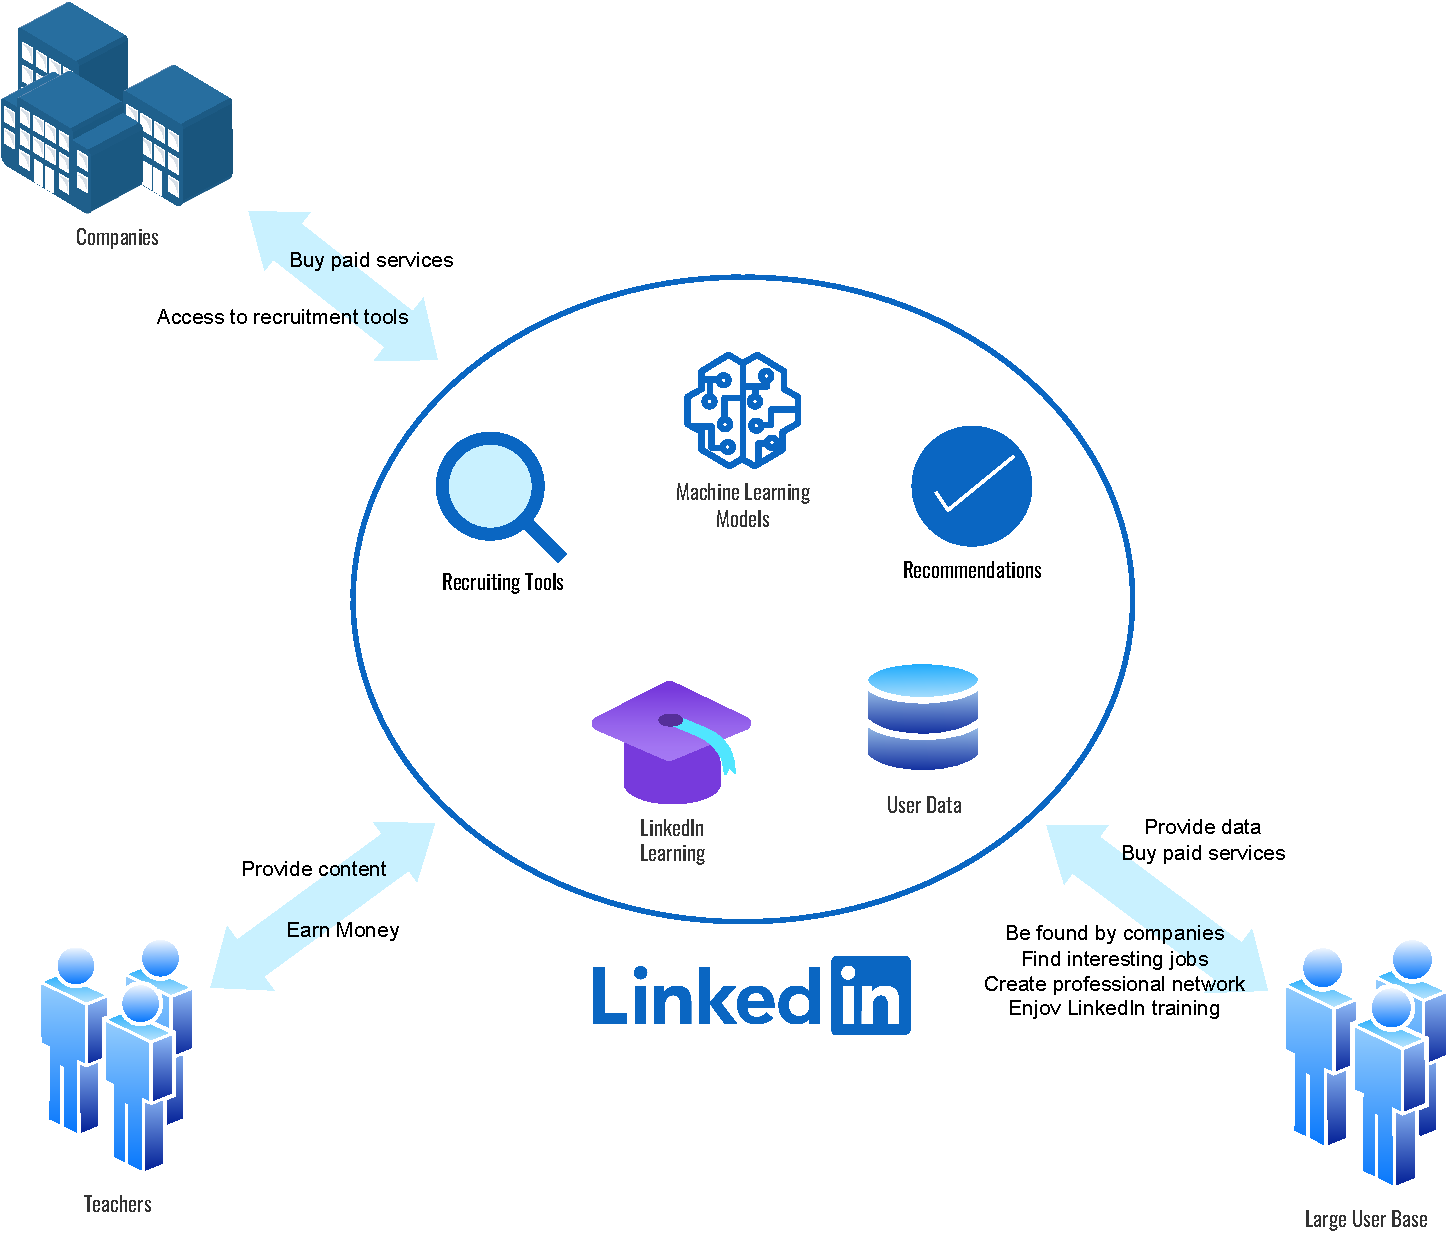
\includegraphics[width=0.76\textwidth]{ecosystem-pre-innovation.pdf}
\end{figure}

According to the definition of digital ecosystems introduced previously, career counseling can not strictly be considered
a digital ecosystem yet. While it meets part of the definition in terms of multilateral relationships between actors, it
fails to meet the criteria of a \textit{set of partners} that pursue a common goal of joint value creation \citep{adnerEcosystemStructureActionable2017}.
The reason for this is that the digital ecosystem of career counseling is not yet a fully integrated ecosystem, but rather
a collection of loosely coupled actors that may also use different platforms for different use cases. The situation of 
career counseling thus presents enormous potential for strategic innovation by bringing all actors together and integrating
them into a fully connected digital ecosystem of career counseling.

A true digital ecosystem could be created by integrating the services of other actors into the LinkedIn ecosystem.
The key idea of the innovation is to add an API layer on top of LinkedIn that allows career counselors to access and leverage
on the data, recommendation engines, and machine learning models deployed by LinkedIn. By using the API layer, the career
counselors can be taken aboard the digital ecosystem. Also, new start-up companies may offer counseling services on top of 
the API layer to the other companies in the ecosystem. By using the API layer, counselors and other participating companies can
participate in the value creation by providing additional, refined data to LinkedIn. LinkedIn can use that data to further
improve the services and train even better machine learning models. For instance, career counselors may provide feedback
on recommendations provided by LinkedIn, which can be used to further refine the recommendation engine. The resulting digital
ecosystem is depicted in Figure \ref{fig:ecosystem-ccaas}. We term this emerging, truly digital ecosystem and business model
\textit{Career-Counseling-as-a-Service} (CCaaS).

\begin{figure}[h!]
    \centering
    \caption{Future state of a true digital ecosystem built around LinkedIn on top of a new CCaaS API layer. Counselors and
    start-ups join the digital ecosystem and participate in the value creation (own illustration).}
    \label{fig:ecosystem-ccaas}
    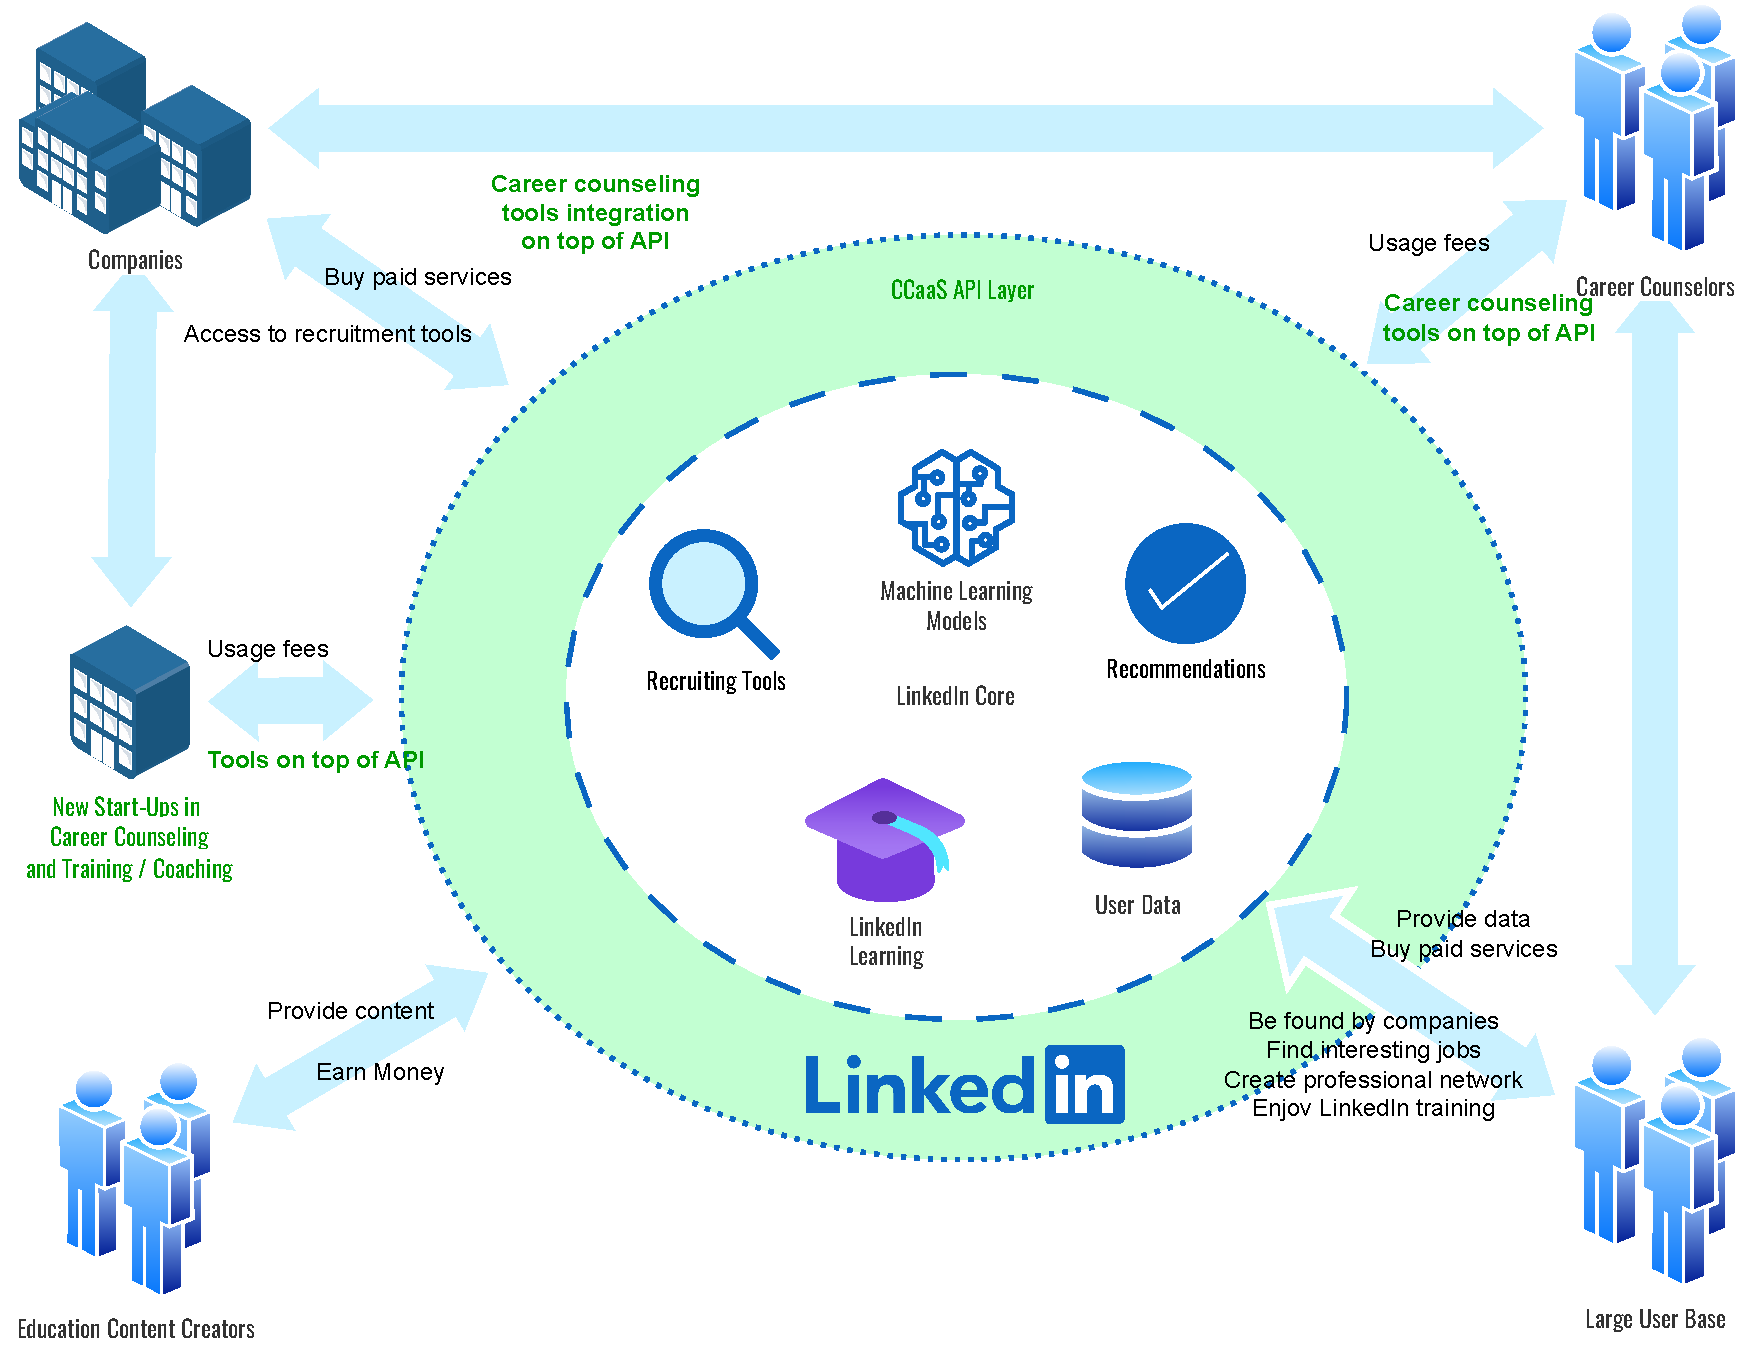
\includegraphics[width=0.8\textwidth]{ecosystem-ccaas.pdf}
\end{figure}

The remainder of this paper will systematically explore the potential of CCaaS by evaluating the business
model in terms of its customer centricity, technical and societal feasibility, economic viability and system fit. 
The next Section \ref{sec:customer_perspective} introduces the customer perspective.
